%% Use the hmcposter class with the thesis document-class option.
\documentclass[thesis]{hmcposter}

\usepackage{graphicx}
\usepackage{natbib}
\usepackage{booktabs}
\usepackage{subfig}
\usepackage{amsmath}
\usepackage{textcomp}
\usepackage{url}
\usepackage{tikz}

\usepackage{import}
\usepackage{xifthen}
\usepackage{pdfpages}
\usepackage{transparent}

\newcommand{\incfig}[1]{%
    \def\svgwidth{0.8 \columnwidth}
    \import{./figures/}{#1.pdf_tex}
}
\newcommand{\mzncar}[3][(0,0)]{
\begin{scope}[shift={#1}]
\shade[top color=#2, bottom color=#3, shading angle=90, draw=white, rounded corners=0.7ex, very thick] (0.75,.25) -- ++(0,0.5) -- ++(0.5,0.15) -- ++(1.5,0) -- ++(0.5,0) -- ++(0,-0.65) -- (0.75,.25) -- cycle;
\draw[thick, rounded corners=0.2ex, fill=white, thick] (1.25,0.85) -- ++(0.5,0.35) -- ++(0.8,0) -- ++(0.3,-0.35) -- (1.25,0.85);
\draw[thick] (2.1,0.85) -- (2.1,1.2);
\draw[fill=gray!80,thin] (1.375,.25) circle[radius=.2];
\draw[fill=gray!80,thin] (2.76,.25) circle[radius=.2];
\end{scope}
}


%% Author of the thesis.
\author{Alan Kappler and Jayden Thadani}

%% The year of your thesis poster's creation.
\posteryear{2024}

%% Thesis Title.
\title{Preference-restricted parking functions}

%% The name of the class for which the poster was created.
%% Generally we see posters for thesis and Clinic, but sometimes
%% other classes require or allow the creation of posters to
%% communicate the results of a project.
%% 
%% Use the format Math nnn: Class Title.
\class{Research in enumerative combinatorics}

%% Advisor(s) name or names.  Separate with \and.
\advisor{Michael Orrison \and Peter Kagey}

%% Define the \BibTeX command, used in our example document.
\providecommand{\bibtex}{{\rmfamily B\kern-.05em%
    \textsc{i\kern-.025em b}\kern-.08em%
    T\kern-.1667em\lower.7ex\hbox{E}\kern-.125emX}}


\pagestyle{fancy}

\begin{document}

\begin{poster}

\section{Classical parking functions}

Imagine $n$ cars drive down a one-way street with $n$ spots. Each car has a favourite parking spot given by $\pi:[n] \to [n]$. In order, the cars try to park: trying their favourite spot, or the next open spot. $\pi$ is a \emph{parking function} if all cars park.

\begin{figure}
    \centering
    \incfig{Parking procedure}
    \caption{The parking procedure for preferences given by $\pi = (2, 1, 2, 2)$}
    \label{fig:parking-procedure}
\end{figure}

\subsection{Enumeration}

Of the $n^n$ possible preference functions for $n$ cars, how many are parking functions? $(n + 1)^{n - 1}$ (magical!) Its circular symmetry proof is even more so!

Is there magic to be found in other questions about parking?

\section{A framework for variants}%

There are many variants of the parking function problem:
\begin{itemize}
\item What if there are more cars than spots? (\cite{cameron-johannsen-prellberg-schweitzer-2008})
\item What if spots can fit multiple cars? (\cite{blake-konheim-1977})
\item The elusive \emph{prime parking functions}
\end{itemize}

These problems can all be modeled by a \emph{preference-restricted parking function} --- a parking function with $\pi([n]) \subset S \subset [n]$.

We can use our intuition for parking functions to solve other parking problems!

\section{$[s]$-restricted parking functions}

Parking functions with $n > s$ cars and $s$ spots are exactly $[s]$-restricted parking functions! All spots will be filled if and only if there are no unfilled spots in the first $s$.

\subsection{Enumeration and Abel's theorem}

How to count? One way: start with all preference functions $[c] \to [s]$ and subtract all those where spots are left empty ---
\[
	s^{n} - \sum_{i = 0}^{s - 1} \binom{n}{i} (i + 1)^{i - 1} (s - i - 1)^{n - i}.
\]

Or, start with all parking functions and sieve out those where cars prefer spots in $[c] \setminus [s]$ ---
\[
	\sum_{i = s}^{n} \binom{n}{i} (i + 1)^{i - 1} (s - i - 1)^{n - i}.
\]

How can we make the sieve work?

Consider parking functions with cars colored red and indigo, where the $i$ indigo cars form a parking function of length $i$ and the remaining red cars prefer the ``forbidden" spots in $[i+1]\backslash [s]$.

For $n=5,s=2,$ for example, we might color the parking function $\pi=(1,3,2,2,4)$ as
\begin{center}
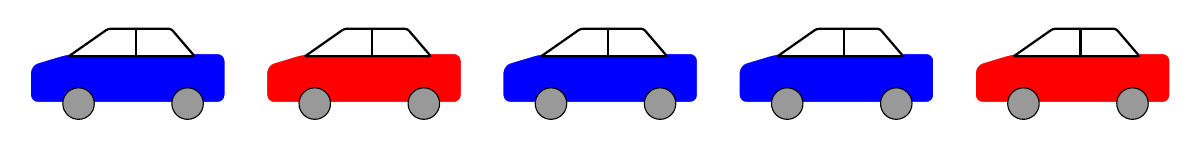
\begin{tikzpicture}
    \mzncar[(0,0)]{blue}{blue} \mzncar[(3,0)]{red}{red} \mzncar[(6,0)]{blue}{blue} \mzncar[(9,0)]{blue}{blue} \mzncar[(12,0)]{red}{red}
\end{tikzpicture}
\end{center}

Counting $i$ even positively and $i$ odd negatively, consider recoloring a car with the largest preference available. For instance, we'd recolor the above as:

\begin{center}
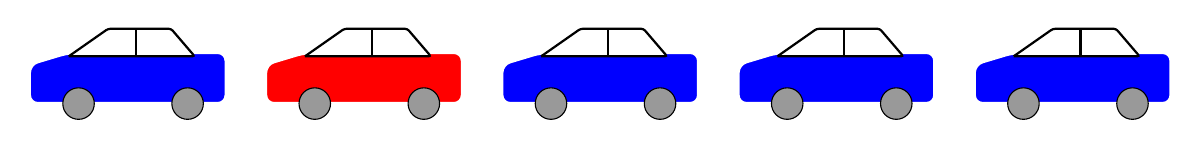
\begin{tikzpicture}
    \mzncar[(0,0)]{blue}{blue} \mzncar[(3,0)]{red}{red} \mzncar[(6,0)]{blue}{blue} \mzncar[(9,0)]{blue}{blue} \mzncar[(12,0)]{blue}{blue}
\end{tikzpicture}
\end{center}

This is nearly an involution, and the only exceptions are when all cars are indigo and have preferences within $[s]$! In our alternating sum, everything cancels except for what we want to count.

These two counts are connected by Abel's generalization of the binomial theorem, which can be recovered from parking functions:
\[
	(x + y + n)^{n} = \sum_{i = 0}^{n} \binom{n}{i} x (x + i)^{i - 1} (y + n - i)^{n - i}.
\]

\newcolumn 
\section{Other restrictions}

\subsection{Modular restrictions}

If $s$ spots can each hold $g$ cars, then we can think about $S$-restricted parking functions for $S = \{ i \in [c] \mid i \equiv 1 \pmod g \}$! \cite{blake-konheim-1977} used complex analysis and generating functions to show that there are $s^{gs - 2}$ ways to park $gs - 1$ cars in this set up. We used a circle argument to give a much simpler proof!

\subsection{Prime parking functions}

Some parking functions can be ``factored'', partitioning the street into intervals on which the preferences form parking functions themselves! The irreducible ones are called ``prime''.

Prime parking functions also have an elegant enumeration and are worth a closer look. They're in bijection with $S$-restricted parking functions for $S = [c]\backslash\{2\}$! The trick is a reshuffling of parking spots: shift all your preferences $n>1$ to $n+1>2.$


\bibliographystyle{hmcmath}
\bibliography{sampleposter}
\vfill

\section{Acknowledgements}

We thank Professors Orrison and Kagey, as well as Jasper Bown '24, for their invaluable guidance and advice throughout the research process. Thank you to the Harvey Mudd Department of Mathematics for supporting this research.

\vfill
\end{poster}

\end{document}



% Let $\pi = (1,2,1,1)$ and ...
% \(
% \begin{tikzpicture}[scale=0.5,baseline=0.3em]
%     \fill[blue] (0,0) rectangle (1,1);
% \end{tikzpicture}
% ~
% \begin{tikzpicture}[scale=0.5,baseline=0.3em]
%     \fill[red] (0,0) rectangle (1,1);
% \end{tikzpicture}
% ~
% \begin{tikzpicture}[scale=0.5,baseline=0.3em]
%     \fill[red] (0,0) rectangle (1,1);
% \end{tikzpicture}
% ~
% \begin{tikzpicture}[scale=0.5,baseline=0.3em]
%     \fill[blue] (0,0) rectangle (1,1);
% \end{tikzpicture}
% \leftrightarrow
% \begin{tikzpicture}[scale=0.5,baseline=0.3em]
%     \fill[blue] (0,0) rectangle (1,1);
% \end{tikzpicture}
% ~
% \begin{tikzpicture}[scale=0.5,baseline=0.3em]
%     \fill[blue] (0,0) rectangle (1,1);
% \end{tikzpicture}
% ~
% \begin{tikzpicture}[scale=0.5,baseline=0.3em]
%     \fill[red] (0,0) rectangle (1,1);
% \end{tikzpicture}
% ~
% \begin{tikzpicture}[scale=0.5,baseline=0.3em]
%     \fill[blue] (0,0) rectangle (1,1);
% \end{tikzpicture}
% \)
